 \documentclass{report}
 
\usepackage[utf8]{inputenc} 
\usepackage[T1]{fontenc}      
\usepackage[top=2.0cm, bottom=3cm, left=3.0cm, right=3.0cm]{geometry}
\usepackage{graphicx}
\usepackage{wrapfig}
\usepackage{amsmath,esint }
\usepackage{amssymb}
\graphicspath{{figures/}{../figures}}

\newcommand*\dif{\mathop{}\!\mathrm{d}}
\newcommand*\diver{\mathop{}\!\mathrm{div}}
\newcommand*\grad{\mathop{}\!\mathrm{grad}}

\begin{document}

\section*{Flux et divergence en coordonnées cylindriques $\bullet\circ\circ$}

On s'intéresse à l'écoulement d'un fluide incompressible en utilisant la description langrangienne. On considère un volume $d\tau$ élémentaire, situé en $P=(r,\theta,z)$ en coordonnées cylindriques. Chaque face de ce volume est indexé de 1 à 6, comme indiqué sur le schéma ci-dessous.

\begin{center}
	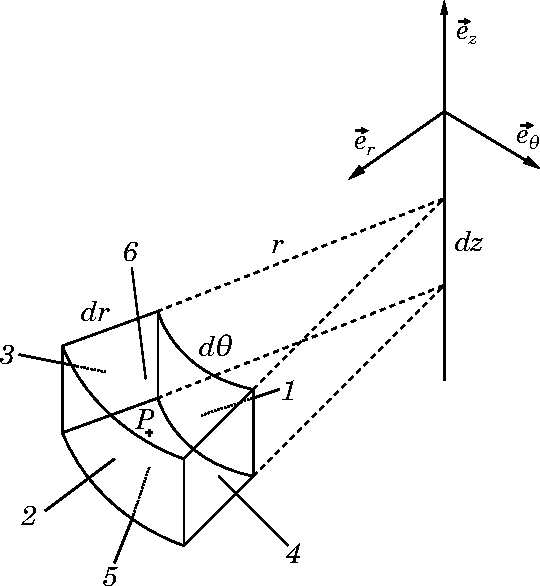
\includegraphics[scale=0.65]{div_meca_flu.pdf}
\end{center}

Le champ de vitesse en tout point $P$ est noté $\vec{v}(r,\theta,z)$. On admet que le débit volumique $\phi_v$ d'un fluide à travers une surface $\Sigma$ est :
\begin{equation}
\label{eq:debit}
	\phi_v = \iint _\Sigma d\vec{S}\cdot\vec{v}
\end{equation}
Plus précisément, c'est la somme sur la surface $\Sigma$ des flux (ou débits volumiques) élémentaires $d\phi_v=d\vec{S}\cdot\vec{v}$.

\begin{itemize}

	\item[$\ast$] Rappeler ce que sont les descriptions langrangienne et eulérienne d'un fluide en écoulement.
	
	\item[$\ast$] Calculer les flux élémentaires $d\phi_{v,i}$ sur chaque face du volume élémentaire $d\tau$, $i\in\{1;6\}$.
	
	\item[$\ast$] En déduire la relation :
	\begin{align*}
	 	\sum_{i=1}^6 d\phi_{v,i} = \mathbf{div}(\vec{v})d\tau
	\end{align*}

	Cela vous rappelle t-il un théorème ?
	
	\item[$\ast$] On suppose désormais que l'écoulement est radial et qu'il ne dépend que de $r$ : $\vec{v}=v(r)\vec{e}_r$. De plus, on suppose que l'écoulement est incompressible, c'est-à-dire que pour tout volume $V$ ne contenant pas l'axe $Oz$, le débit de fluide entrant dans $V$ est égal au débit de fluide sortant.
	
	En déduire que le champ de vitesse s'écrit $\vec{v}=\frac{A}{r}\vec{e}_r$, où $A$ est constante.
	
	\item[$\ast$] On s'intéresse au volume $V$ délimitant un cylindre coaxial à l'axe $Oz$, de hauteur $h$, de rayon $R$. En considérant le champ de vitesse radial de la question précédente, calculer le débit volumique $\phi_v$ s'écoulant à travers les parois de ce cylindre en utilisant la définition du débit donné avec la formule $\ref{eq:debit}$. Est-ce compatible avec le théorème de Green-Ostrogradski ?
	
\end{itemize}

\textit{Données}

Divergence en coordonnée cylindrique d'un vecteur $\vec{A}$ :
\begin{align*}
\mathbf{div}(\vec{A})=\frac{1}{r}\frac{\partial (r A_r)}{\partial r} + \frac{1}{r}\frac{\partial A_\theta}{\partial \theta} + \frac{\partial A_z}{\partial z}
\end{align*}

Théoèreme de Green-Ostrogradski :
\begin{align*}
\int\!\!\!\!\!\int\!\!\!\!\!\int_{V} \mathbf{div}(\vec{A})\, {\rm d}\tau =
\int\!\!\!\!\!\!\!\subset\!\!\!\supset\!\!\!\!\!\!\!\int_{\Sigma}  \overrightarrow A \cdot \mathrm d \overrightarrow{S}
\end{align*}

\newpage

\section*{Embouteille sur une autoroute}

Sur une autoroute à 3 voies, la circulation est fluide, les véhicules se répartissent sur les 3 voies, se suivent sur chaque voie à 200m d'écart et se déplacent à $v_0=$30$m.s^{-1}$ en moyenne. Un bouchon routier se forme subitement au point kilométrique $D$. Dans le bouchon, les véhicules sont à l'arrêt à raison d'un véhicule dans un espace de 10m de long en moyenne. Déterminer la vitesse du front du bouchon.

\newpage

\section*{Forme d'une coulée d'huile}

Un bidon d'huile est muni d'une ouverture circulaire de rayon $R$ et de centre $O$, à travers laquelle l'huile tombe et s'écoule en régime permanent. On définit l'axe vertical $Oz$ dirigé vers le bas et on note $\vec{g}=g\vec{e}_z$ l'accélération de la pesanteur, la masse volumique de l'huile $\mu$, et le débit massique sortant $D$. A la côte $z$, la vitesse du fluide $\vec{v}=v(z)\vec{e}_z$ est supposée uniforme. A l'ouverture en $z=0$, l'huile a une vitesse $v_0$. Une fois sortie, la vitesse de l'huile $v(z)$ est prise égale à celle qu'aurait une bille en chute libre sans frottement lachée en $z=0$ avec une vitesse $v_0$. 

\begin{itemize}

	\item[$\curlyvee$] Donner l'expression de $v_0$ en fonction de $\mu$, $D$ et $R$.
	
	\item[$\curlyvee$] Etablir l'expression de $v(z)$.
	
	\item[$\curlyvee$] Déterminer le rayon $r(z)$ du filet d'huile à la côté $z$. On pourra simplifier l'expression finale en supposant $v_0\simeq0$.
	
	\item[$\curlyvee$] Calculer le terme $\vec{v}\cdot\mathbf{grad}(\vec{v})$. Que représente t-il (on rappelle que l'écoulement est stationnaire) ? En déduire la vitesse $\vec{V}$ d'une particule de poussière contenue dans l'huile lors de l'écoulement. Préciser ce que sont les descrptions lagrangiennes et eulériennes d'un fluide.
	
	\item[$\curlyvee$] Le bidon est à une hauteur $H$ du sol. On referme rapidement l'ouverture du bidon. Quelle est la masse d'huile qui reste à s'écouler sur le sol ?

\end{itemize}

\newpage

\section*{\textit{Correction - Forme d'une coulée d'huile}}

\begin{itemize}

	\item[$\curlyvee$] On a tout simplement $v_0=D/(\pi R^2\mu$.
	
	\item[$\curlyvee$] On utilise le théorème de Bernouilli (ou le fait que c'est une chute libre, comme dit dans l'énoncé, ce qui revient au même) :
	\begin{align*}
	\frac{v_0^2}{2} - \frac{v^2(z)}{2} = -gz
	\end{align*}
	donc $v(z)=\sqrt{v_0^2+2gz}$.
	
	\item[$\curlyvee$] Conservation du débit : $D=\mu v(z)\pi r^2(z)$, donc :
	\begin{align*}
		r(z)&=\sqrt{\frac{D}{\mu \pi \sqrt{v_0^2+2gz}}}\\
		&\simeq\sqrt{\frac{D}{\mu\pi\sqrt{2g}}}z^{-\frac{1}{4}}
	\end{align*}
	
	\item[$\curlyvee$] Le terme se résume ici à : $\vec{v}\cdot\mathbf{grad}(\vec{v})=v_z\frac{\partial v_z}{\partial z}=g$. Il représente l'accélération convective, c'est-à-dire à un changement du champ de vitesse dans l'espace, qui est non-nulle malgré le caractère permanent de l'écoulement. L'accélération $\dot{V}(t)$ de la particule de poussière correspond à l'altitude $z$ à ce terme d'accélération convective. Il s'agit tout simplement d'une chute libre (aussi).
	
	\item[$\curlyvee$] La masse d'huile qui continue à se répandre est celle contenue dans la colonne en chute de hauteur $H$. Elle correspond à :
	\begin{align*}
		M=&\int_0^Hdz\mu \pi r^2(z) \\
		=&\frac{D}{\sqrt{2g}}\int_0^Hdzz^{-\frac{1}{2}}\\
		=&D\sqrt{\frac{2H}{g}}
	\end{align*}

\end{itemize}

\newpage

\section*{Résistance autour d'une bille $\bullet\bullet\circ$}

On s'intéresse à l'écoulement stationnaire, incompressible d'un fluide de masse volumique $\rho$ et de viscosité $\eta$ autour d'une sphère de rayon $R$. La vitesse de l'écoulement loin de la sphère est $v_\infty\vec{e_z}$. On adoptera les coordonnées sphériques d'axe $Oz$, $O$ étant le centre le centre de la sphère. 

\begin{itemize}
	\item[•] On suppose que l'écoulement permet de négliger le terme convectif de l'équation de Navier-Stokes devant le terme diffusif. Comment s'écrit alors cette équation ? 
	\item[•] On suppose que la vitesse est telle que : $\vec{rot}(\vec{rot}(\vec{v}))=\frac{3v_\infty R}{r^3}\left(\cos\theta\vec{e_r}+\frac{1}{2}\sin\theta\vec{e_\theta} \right) $. Quelle est la résultante des forces de pression sur la sphère ? 
	\item[•] Quelle est la résultante des actions de cisaillement sur la sphère ? On donne $\left(\frac{\partial v_\theta}{\partial r}\right)_{r=R}=\frac{3v_\infty}{2R}\sin\theta  $.
	\item[•] Trouver la force de trainée s'exerçant sur la sphère. 
\end{itemize}

On donne : 
\begin{equation}
	\Delta f = \frac{1}{r^2}\frac{\partial}{\partial r} \left(r^2\frac{\partial f}{\partial r} \right) + \frac{1}{r^2\sin\theta}\frac{\partial}{\partial \theta} \left(\sin\theta\frac{\partial f}{\partial \theta} \right) + \frac{1}{r^2\sin^2\theta}\frac{\partial^2 f}{\partial \varphi^2} 
\end{equation}

\begin{equation}
	\vec{grad} f = \frac{\partial f}{\partial r} \vec{e_r} + \frac{1}{r}\frac{\partial f}{\partial \theta}\vec{e_\theta} + \frac{1}{r\sin\theta}\frac{\partial f}{\partial \varphi}\vec{e_\varphi}
\end{equation}

\newpage

\section*{Ecoulement d'un fluide en pente $\bullet\circ\circ$}

On considère un fluide d'épaisseur $h$ s'écoulant lentement sur un plan infini incliné d'un angle $\alpha$ par rapport à la verticale. Le fluide a une forte viscosité $\eta$ et une masse volumique $\rho$, et il est soumis à la gravité. On est en régime permanent, et on suppose que la vitesse selon $\vec{e}_y$ est nulle.

\begin{center}
	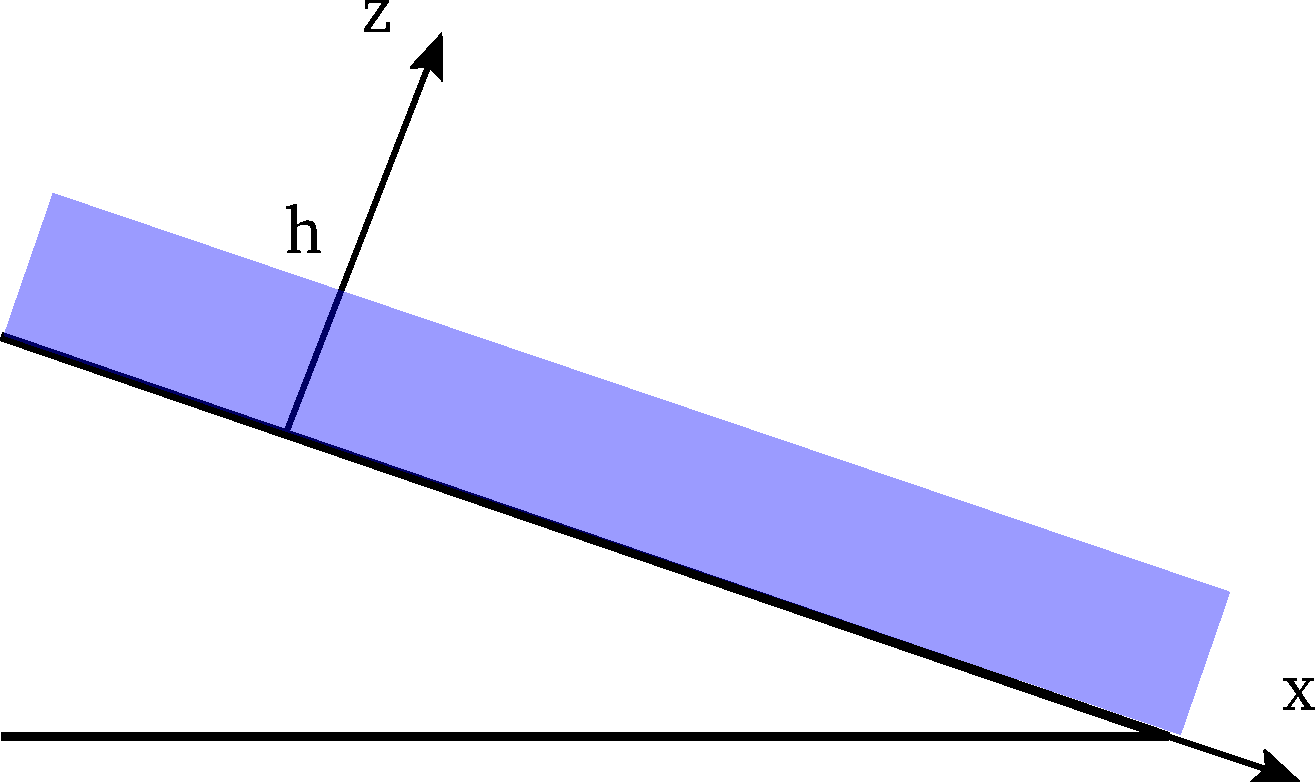
\includegraphics[scale=0.3]{ecoulement.pdf}
\end{center}

\begin{itemize}

	\item[$\blacktriangleright$] Ecrire le bilan des forces volumiques s'exerçant sur un volume de fluide situé au point $M=(x,y,z)$.
	\item[$\blacktriangleright$] Montrer que $\vec{v}(x,y,z)=v(z)\vec{e_x}$. Quel est le profil de vitesse dans le fluide ? 
	\item[$\blacktriangleright$] En déduire le débit linéique (le débit par unité de longueur selon l'axe $y$).
	\item[$\blacktriangleright$] On souhaite avoir un ordre de grandeur de la viscosité d'un glacier. Pour cela, dispose d'image satellite du glacier du Tacul, situé sur la face nord du Mont Blanc. Chaque "rayure" correspond à une année. Estimer sa viscosité. 
	
\begin{center}
	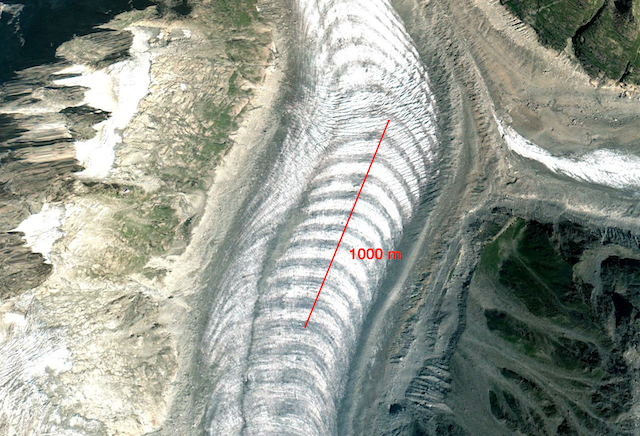
\includegraphics[scale=1]{glacier.png}
\end{center}


	\item[$\blacktriangleright$] En reprenant la première figure, on place désormais une plaque au dessus du liquide, au niveau de $z=h$. Que deviennent les conditions aux limites ? Trouver le nouveau profil de vitesse. Comment s'appelle se type d'écoulement ?

\end{itemize}

\newpage

\section*{Exercice 3}

On étudie un écoulement permanent d'un fluide incompressible de masse volumique $\mu$, dans un tuyau cylindrique horizontal d'axe $Oz$, de rayon $R$, et de longueur $L$ (schéma de gauche). Le champ de pression appliqué le long du tube est noté $P(r,z)$. Par invariance, le champ de vitesse est supposé ne dépendre que de $r$ et $z$, et est dirigé selon $\vec{e_z}$. Il est noté $\vec{u}=u(r,z)\vec{e_z}$. On définit la vitesse de cisaillement par la quantité $\dot{\gamma}=-\frac{du}{dr}$. 

\begin{center}
	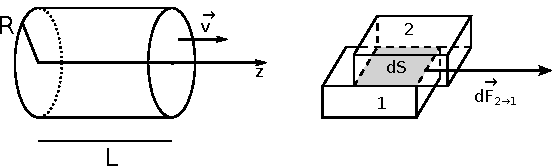
\includegraphics[scale=0.8]{meca_flu2.pdf}
\end{center}

On définit la force surfacique de viscosité $\vec{\tau}$, ou contrainte de cisaillement, entre deux couches adjacentes de fluide, la quantité : $\vec{\tau}=\frac{d\vec{F}}{dS}$.
où $d\vec{F}$ est la force qui s'exerce mutuellement entre les couches adjacentes, et $dS$ la surface élémentaire de contact entre ces deux surfaces (schéma de droite).

\begin{itemize}
	\item[$\bigstar$] Quelle est la relation entre la force de viscosité $\vec{\tau}$ et le champ de vitesse $u$ dans le cas d'un fluide classique (vu en cours), dit newtonien ? On pourra dans cette question se placer en coordonnées cartésiennes.
	
\end{itemize}

\subsubsection*{Fluide de Bingham}

Un fluide est dit de Bingham si les contraintes de cisaillements entre les couches obéissent à une loi de seuil : 
\begin{align*}
	\left\lbrace
\begin{array}{ccc}
\tau>\tau_s & : & \tau = \tau_s+\eta\dot{\gamma} \\
\tau<\tau_s & : & \dot{\gamma}=0\\
\end{array}\right.
\end{align*}
On supposera que le fluide que l'on étudie obéit à une telle loi. 

\begin{itemize}
	\item[$\bigstar$] Quel est la différence entre un fluide classique et un fluide de Bingham ?

	\item[$\bigstar$] Montrer que $\vec{u}$ ne dépend que de $r$. En négligeant les actions de la pesanteur, déterminer la relation suivante : 
	\begin{align*}
		\frac{\partial P}{\partial z} + \frac{1}{r}\frac{\partial (r\tau)}{\partial r}=0
	\end{align*}
	\item[$\bigstar$] Établir la relation :
	\begin{align*}
		\tau(r) = \tau_s\frac{r}{R_s}
	\end{align*}
	où $R_s$ est le rayon de seuil, défini par $R_s=2\tau_s L/\Delta P$, en notant $\Delta P = P(0)-P(L)$ la chute de pression entre l'entrée et la sortie du tuyau. Quel est le signe de $\Delta P$ ?

	\item[$\bigstar$] Pour quelle pression minimale $\Delta P_{min}$ commence t-on à voir un écoulement à travers le tube ?
	
	\item[$\bigstar$] On suppose que $\Delta P>\Delta P_{min}$. Déterminer le champs de vitesse dans le tube. Tracer son allure et expliquer pourquoi l'écoulement présente une zone dite \textit{bouchon}.
	
	
\end{itemize}

\newpage

\section*{Exercice 4}

\subsubsection*{Tuyau parabolique}

Un fluide est en écoulement permanent dans une portion de tube à section parabolique, avec $Oz$ en axe de symétrie. Les lignes de courant s'écoulant dans le tube ont pour équation :
\begin{align*}
		\left\lbrace
\begin{array}{ccc}
z<0 & : & r=\lambda a \\
z>0 & : & r=\lambda \left(a+\frac{z^2}{b} \right) \\
\end{array}\right.
\end{align*}
où $a$ est le rayon du tube pour $z<0$ et $b$ une longueur caractrsitique de l'évasement du tube pour $z>0$ (cf schéma). Le paramètre $\lambda$ décrit permet de décrire les lignes de courant : chaque ligne de courant est paramétrée par une valeur de $\lambda$ donné.

\begin{center}
	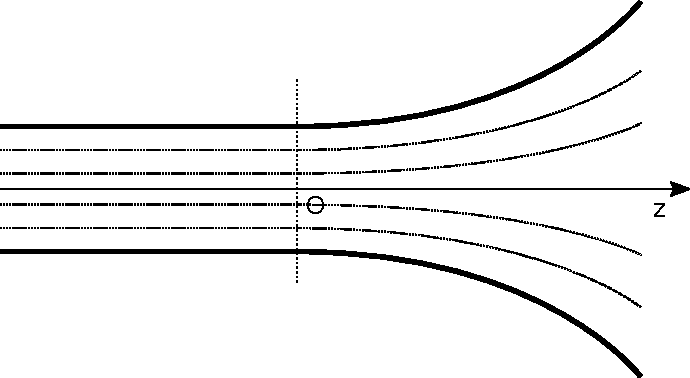
\includegraphics[scale=0.5]{meca_flu1.pdf}
\end{center}

Le fluide est incompressible et la composante axiale de $v_z$ de la vitesse est supposée uniforme sur une section perpendiculaire, cad $v_z$ ne dépend pas de $r$. On note $v_0$ la vitesse en $O$.

\begin{itemize}
	\item[$\ast$] Déterminez la composante vitesse selon $z$, $v_z$ en tout point. 
	\item[$\ast$] Déterminez la composante vitesse selon $r$, $v_r$ en tout point. En déduire l'expression du champ de vitesse $\vec{v}$.
	\item[$\ast$] Comment évolue un élément de fluide qui traverse le tuyau ? 
	\item[$\ast$] Un écoulement est dit rotationnel si une particule de fluide ne subit pas de rotation lors de l'écoulement. Est-ce le cas ici ? On pourra le vérifier en calculant $\mathrm{\vec{rot}} (\vec{v})$ : si $\mathrm{\vec{rot}} (\vec{v})\neq0$ alors l'écoulement est irrotationnel. On donne la formule du rotationnel en coodronnées cylindrique ci-dessous.
	
\end{itemize}

\begin{align*}
	\mathbf{rot} \mathbf{A}
   = \left(\frac{1}{r}\frac{\partial \mathrm{A}_z}{\partial \theta} - \frac{\partial \mathrm{A}_\theta}{\partial z}\right) \mathbf{u_r}
   + \left(\frac{\partial \mathrm{A}_r}{\partial z} - \frac{\partial \mathrm{A}_z}{\partial r}\right)\mathbf{u_\theta}
   + \frac{1}{r}\left(\frac{\partial}{\partial r}(r \mathrm{A}_\theta) - \frac{\partial \mathrm{A}_r}{\partial \theta}\right) \mathbf{u_z}
\end{align*}

\subsubsection*{Écoulement entre deux lames}

On considère deux plaques infinies de verres séparées d'une épaisseur $e$ où circule un fluide incompressible. Du fluide est injecté à un débit $D_e$ par le tuyau $A$, et il peut ressortir à travers le tuyau $B$ identique. On suppose que l'écoulement est incomprésible et relativement lent.

\begin{center}
	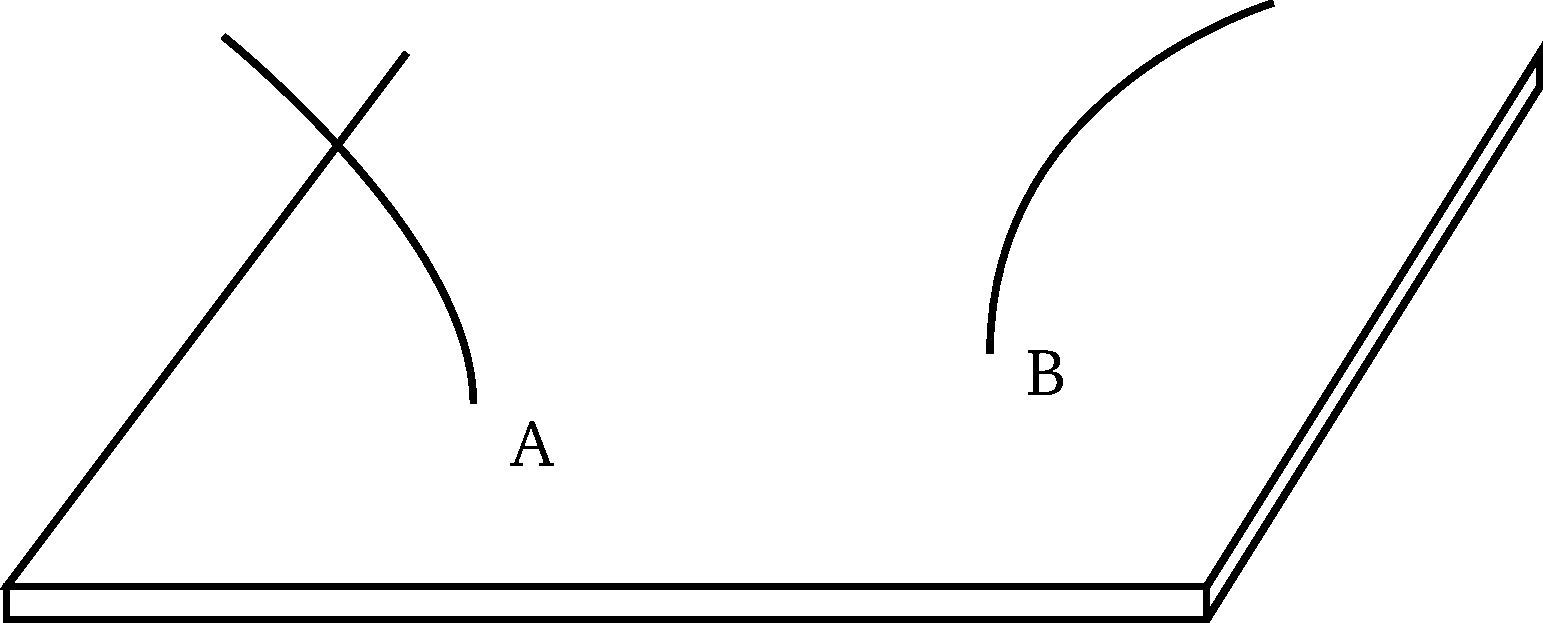
\includegraphics[scale=0.25]{plaque.pdf}
\end{center}

\begin{itemize}
	\item[1 - ] Proposer une solution pour le champ de vitesses en faisant des hypothèses raisonnables.
	\item[2 - ] Est-ce un écoulement compressible ?
\end{itemize}

\newpage

\section*{Boîte automatique $\bullet\bullet\bullet$}

On s'intéresse au convertisseur de couple d'une boite automatique d'un véhicule, qui permet de se passer d'un embrayage. On le modélise comme un système de deux cylindres de même axe $\vec{e}_z$, et de rayons respectifs $R_1$ et $R_2$, de longueur $L$, où se trouve un fluide de viscosité $\eta$ élevée (\textit{schéma de gauche}). Le moteur (respectivement l'arbre de transmission) est solidaire du cylindre $1$ (resp. 2) et tourne à la vitesse $\Omega_1$ (resp. $\Omega_2$). Lorsque le moteur fournit un couple $\Gamma_1$ au cylindre 1, il entraîne le fluide situé entre $R_1$ et $R_2$, qui entraîne à son tour le cylindre 2. On souhaite étudier le fonctionnement du dispositif, et pour cela, on se placera en coordonnées cylindriques. 

\begin{center}
	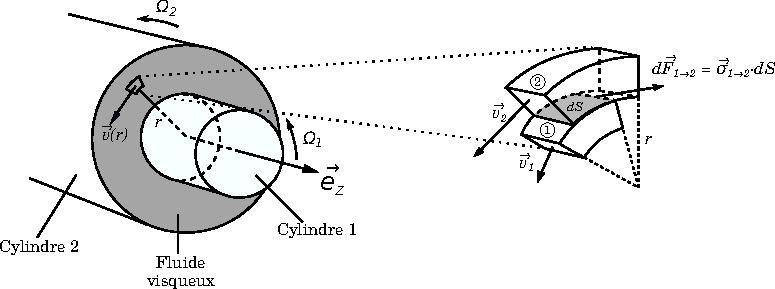
\includegraphics[scale=0.8]{boite_auto.pdf}
\end{center}

On rappelle que la force surfacique de viscosité, entre deux couches élémentaires 1 et 2 adjacentes de fluide, s'écrit : $\vec{\sigma}_{1\rightarrow2}=\frac{d\vec{F}_{1\rightarrow2}}{dS}$, où $d\vec{F_{1\rightarrow2}}$ est la force exercée de la couche 1 sur la couche 2,  $dS$ étant la surface élémentaire de contact (\textit{schéma de droite}). On admet que son expression en coordonnées cylindriques de sa composante selon $\vec{e_\theta}$ s'écrit : 
\begin{align*}
	\sigma_\theta(r,\theta,z)=\eta\left(\frac{1}{r}\frac{\partial v_r}{\partial \theta}+ \frac{\partial v_\theta}{\partial r} - \frac{v_\theta}{r} \right)
\end{align*}

On admet que les autres composantes de $\vec{\sigma}$ sont nulles ($\sigma_r=\sigma_z=0$). On suppose par ailleurs que l'écoulement est permanent, que la vitesse ne dépend que de $r$, et enfin que $v_z=0$.

\begin{itemize}
		
	\item[$\bigstar$] Quel est le nombre de Reynolds de cet écoulement ? En déduire le type d'écoulement. 
	
	\item[$\bigstar$] Montrer que le champ de vitesse est strictement orthoradial : $\vec{v}=v_\theta (r)\vec{e_\theta}$.
	
	\item[$\bigstar$] En faisant un bilan des moments sur un élément de fluide selon $\vec{e_z}$ et en négligeant les forces de pression, montrer que la vitesse vérifie la relation suivante : 
	\begin{align*}
		\frac{\partial}{\partial r}\left(r^3 \frac{\partial}{\partial r}\frac{v_\theta}{r} \right) =0
	\end{align*}
	
	\item[$\bigstar$] A l'aide des conditions aux limites, en déduire l'expression du champ de vitesse $\vec{v}$.
	
	\item[$\bigstar$] Calculer le couple $\Gamma_{1\rightarrow2}$ qu'exercent les forces visqueuses sur le cylindre 2. Comparer avec $\Gamma_{2\rightarrow1}$.
	\end{itemize}

On suppose que le moteur peut asservir son régime moteur de sorte à garder $\Omega_1$ fixé, quelque soit le couple $\Gamma_{1\rightarrow2}$ qu'il délivre.

\begin{itemize}
	
	\item[$\bigstar$] Le véhicule roule à vitesse constante dans une montée, équivalent à un couple résistif $-\Gamma_r$ sur l'arbre de transmission. Déterminer $\Omega_2$ puis le rendement du convertisseur de couple. Quels sont les intérêts et les incovénients d'un convertisseur de couple par rapport à un embrayage classique ?
	
	\item[$\bigstar$]  Désormais, le véhicule est intialement à l'arrêt, et démarre à pleine puissance sur une route plate à $t=0$. L'inertie du véhicule est vue au niveau du cylindre 2 comme un moment d'inertie $J$. Déterminer l'évolution $\Omega_2(t)$. 
		
\end{itemize}

\textit{Données :} $R_1=295$mm, $R_2=300$mm, $L=500$mm, $\rho=860$kg.m$^{-3}$ et $\eta=120$ SI. 
\begin{align*}
	\mathrm{div}(\vec{A}) =
\frac{1}{r}\frac{\partial (r A_r)}{\partial r} + \frac{1}{r}\frac{\partial A_\theta}{\partial \theta} + \frac{\partial A_z}{\partial z}
\end{align*}	

\newpage

\section*{Exercice 5}

On considère un fluide incompressible, de viscosité $\eta$ contenu entre deux cylindres orientés verticalement, de même axe $O_z$, et de rayons respectifs $R_1$ et $R_2$ (avec $R_1<R_2$). La hauteur des cylindres $L$ est très grande devant les rayons : $L\gg R_1, R_2$. Les deux cylindres peuvent tourner indépendamment l'un de l'autre autour de l'axe $Oz$. 

\begin{center}
	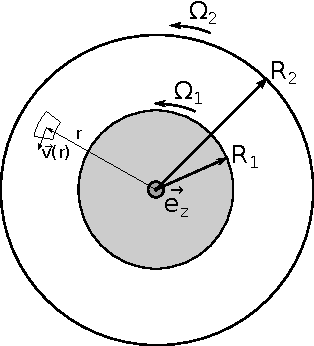
\includegraphics[scale=0.8]{meca_flu3.pdf}
\end{center}

On définit la force surfacique de viscosité $\vec{\sigma}$, ou contrainte de cisaillement, entre deux couches élémentaires adjacentes de fluide, la quantité : $\vec{\sigma}=\frac{d\vec{F}}{dS}$,
où $d\vec{F}$ est la force qui s'exerce mutuellement entre les couches adjacentes, et $dS$ la surface élémentaire de contact entre ces deux surfaces. L'expression en coordonnées cylindrique de sa composante selon $\vec{e_\theta}$ s'écrit : 
\begin{align*}
	\sigma_\theta(r,\theta,z)=\eta\left(\frac{1}{r}\frac{\partial v_r}{\partial \theta}+ \frac{\partial v_\theta}{\partial r} - \frac{v_\theta}{r} \right)
\end{align*}
Il est possible de démontrer que, dans le cadre de ce problème, les autres composantes de $\vec{\sigma}$ sont nulles : $\sigma_r=\sigma_z=0$. Nous l'admettrons pour la suite du problème. 

L'écoulement est supposé permanent. On suppose aussi que $v_z=0$.

\begin{itemize}
	\item[$\clubsuit$] Quel est le nombre de Reynolds de cet écoulement ? En déduire le type d'écoulement. \textit{Données :} $R_1=40$cm, $R_2=60$cm, $\Omega_1\simeq\Omega_2=1$rad.s$^{-1}$, $\rho=960$kg.m$^{-3}$ et $\eta=120$ SI. 

	\item[$\clubsuit$] A partir des invariances du problèmes, montrer que $v$ ne dépend que de $r$. En s'appuyant sur un bilan de matière, retrouver l'expression de l'équation de conservation de la masse (ou du débit) et en déduire que le champ de vitesse s'écrit $\vec{v}=v_\theta (r)\vec{e_\theta}$.
	
	\item[$\clubsuit$ ] En faisant un bilan des moments sur un élément de fluide selon $\vec{e_z}$, montrer que la vitesse vérifie la relation suivante : 
	\begin{align*}
		\frac{\partial}{\partial r}\left(r^3 \frac{\partial}{\partial r}\frac{v_\theta}{r} \right) =0
	\end{align*}
Pourquoi les forces de pression n'interviennent-elles pas ?	
	
	\item[$\clubsuit$] Le cylindre de rayon $R_1$ (resp. $R_2$) tourne à la vitesse angulaire $\Omega_1$ (resp. $\Omega_2$). En déduire l'expression du champs de vitesse. 
	
	\item[$\clubsuit$ ] On suppose que le cylindre intérieur (de rayon $R_1$) est maintenu fixe (cad $\Omega_1=0$) à l'aide d'un ressort de torsion qui exerce un moment $\vec{M}=k\theta\vec{e_z}$. Le cylindre extérieur tourne toujours à la vitesse $\Omega_2$. De quel angle $\theta$ tourne le ressort ? A quel quantité physique a t-on alors accès ?
	
	\item[$\clubsuit$ ] En étant toujours dans la situation $\Omega_1=0$, calculer la puissance mécanique dissipée dans le fluide.
	
\textit{NB :} 
\begin{align*}
	\mathrm{div}(\vec{A}) =
\frac{1}{r}\frac{\partial (r A_r)}{\partial r} + \frac{1}{r}\frac{\partial A_\theta}{\partial \theta} + \frac{\partial A_z}{\partial z}
\end{align*}	
	
\end{itemize}

\newpage

\section*{Exercice 6}

Une tornade assimilée à un écoulement parfait, permanent, incompressible de l'air, de masse volumique $\mu = 1.3$kg.m$^{-3}$, est caractérisé par un vecteur tourbillon $\vec{\Omega} = \Omega \vec{u_{z}}$, supposé uniforme à l'intérieur de la tornade ($r\leq a$) et nul à l'extérieur de la tornade. Cette dernière est modélisée par un cylindre d'axe ($Oz$) et de rayon $a=50$m. On se place en coordonnées cylindriques.

\begin{itemize}

	\item[1 - ] Donnez une expression intégrale de la vitesse $\vec{v}$ (on ne cherche pas à calculer cette intégrale à ce stage de l'exercice). A quel problème électrostatique la tornade est-elle assimilable ?
	\item[2 - ] On se limite à des mouvements de l'air définis par $\vec{v} = v(r)\vec{u_{\theta}}$. Donner l'allure de $v(r)$.
	\item[3 - ] Calculer le champ de pression. On rappelle que : 
	\begin{align*}
		(\vec{v}.\vec{grad})\vec{v} =\vec{grad}(v^{2}/2) + 2\vec{\Omega}\wedge \vec{v}
	\end{align*}
	\item[4 - ] Quelle est la vitesse maximale théorique que peut avoir une tornade ? Est-ce physiquement possible ?
	\item[4 - ] Un toit de masse surfacique de $100$kg.m$^{-2}$, simplement posé et horizontal, peut être soulevé au passage de la tornade ? On suppose que la vitesse maximale de la tornade est $v_{max} = 180$km.h$^{-1}$.
\end{itemize}

On donne :

\begin{align*}
	div\vec{A} = \frac{1}{r}\frac{\partial(rA_{r})}{\partial r} +\frac{1}{r}\frac{\partial A_{\theta}}{\partial\theta} + \frac{\partial A_{z}}{\partial z}
\end{align*}
\begin{align*}
	\vec{grad}U = \frac{\partial U}{\partial r}\vec{e}_{r} +\frac{1}{r}\frac{\partial U}{\partial\theta}\vec{e}_{\theta} + \frac{\partial U}{\partial z}\vec{e}_{z}
\end{align*}

\newpage

\section*{Exercice 7}

Le tube en "L" suivant a une section constante $s$, mais dont les dimensions longitudinales sont très grande devant le diamètre, on pourra considérer que l'écoulement est unidimensionnel. Le liquide est supposé idéal et incompressible.

Dans l'état initial, la hauteur du liquide est $h_0$ et l'extrémité inférieur est bouchée. On ouvre le bouchon à $t=0$.

\begin{center}
	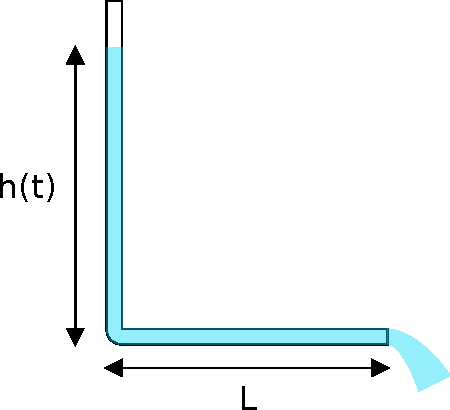
\includegraphics[scale=0.5]{meca_flu4.pdf}
\end{center}

\begin{itemize}

\item[1 - ] Déterminez la vitesse d'éjection $v$ en fonction la hauteur $h$. Examiner le cas où $L\longrightarrow0$.

\item[2 - ] Exprimer la pression $P(M,t)$ en tout point en fonction de $P_{atm}$, $\rho$, $g$, $L$ et $h(t)$. En quel point est-elle maximale ?

\end{itemize}

\newpage

\section*{Exercice 8}

\begin{wrapfigure}[12]{r}{4cm}
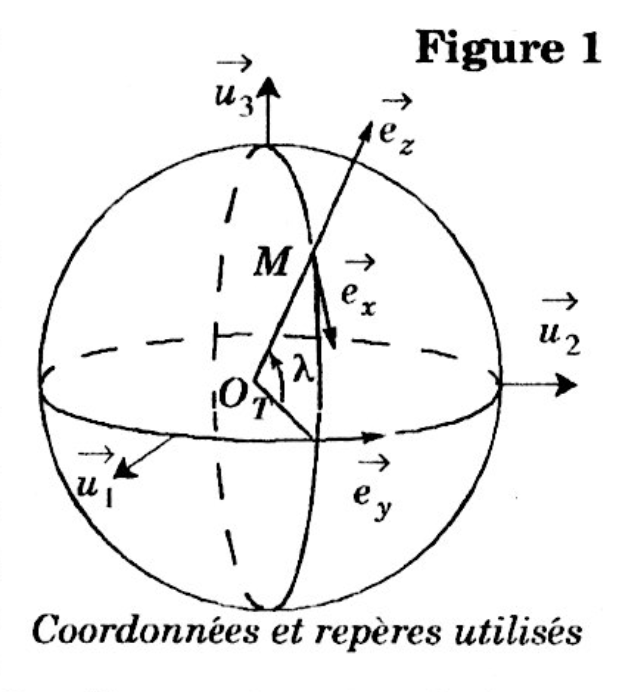
\includegraphics[width=4cm]{meca_flu5.png}
\end{wrapfigure}

On considère la Terre comme une sphère de rayon $R_T$ et de centre $O_T$. Le repère $R_G=(\vec{u_1},\vec{u_2},\vec{u_3})$ est fixe et est considéré comme galiléen, avec $\vec{u_3}$ parallèle à l'axe Nord-Sud. Pour tout point $M$ de latitude $\lambda$ de la surface, on associe le repère $R_T=(\vec{e_x},\vec{e_y},\vec{e_z})$. Ce repère $R_T$ est donc en rotation $\vec{\Omega}=\Omega\vec{u_3}$ par rapport à $R_G$.


On note $\vec{g}$ le champ de pesanteur terrestre. L'atmosphère est considéré comme une fine couche d'air, qui est un gaz parfait de masse molaire $M$, de masse volumique $\rho$, et dont les écoulements sont considérés comme parfaits. On notera $v(x,y,z)$ le champ des vitesses dans $R_T$, $P(x,y,z)$ le champ de pression.

On cherche à étudier les vents dominants à la surface du globe, cad on se limite aux écoulements de grande échelle, réguliers dans le temps (stationnaires). 

\begin{itemize}

	\item[$\clubsuit$] Le référentiel $R_T$ n'étant pas galiléen, on admet que les forces volumiques d'inertie se réduisent au terme de Coriolis, qui s'écrit : $f_{vol, C}=-2\rho\vec{\Omega}\wedge\vec{v}$. Comment s'écrit la relation fondamentale de la dynamique ?
	
	\item[$\clubsuit$] En faisant l'hypothèse que l'atmosphère est isotherme, et en supposant que l'air est à l'équilibre (cad dans fixe par rapport à $R_T$), estimer l'épaisseur de l'atmosphère. On notera $P_{eq}(x,y,z)$ la pression correspondante. Que peut-on en déduire sur la partie verticale de la vitesse $v_z=\vec{v}\cdot\vec{e_z}$ ?
	
	\item[$\clubsuit$] En notant $p(x,y,z)=P(x,y,z)-P_{eq}(x,y,z)$, trouver la nouvelle relation vérifiée par $\vec{v}$ et $p(x,y,z)$
	
	\item[$\clubsuit$] On appelle nombre de Rossby (noté $Ro$) d'un écoulement le rapport entre le terme d'accélération particulaire et l'accélération lié à la force de Coriolis. Estimer $Ro$ pour des mouvements atmosphériques où la vitesse typique est $U\simeq10$m.s$^{-1}$ et d'extension $L\simeq1000$km. Simplifier l'équation trouvée à la première question.
	
	\item[$\clubsuit$] Établir alors l'expression du champs de vitesse $\vec{v}$. Pourquoi seule la composante horizontale de $\vec{grad}(p)$ intervient dans l'expression de $\vec{v}$ ?
	
	\item[$\clubsuit$] La figure ci dessous donne la valeur moyenne de la pression atmosphérique $P$ au niveau du sol, le long d'un méridien quelconque. En déduire l'allure de la circulation des vents sur le globe, en fonction de la latitude $\lambda$.
	
\begin{center}
	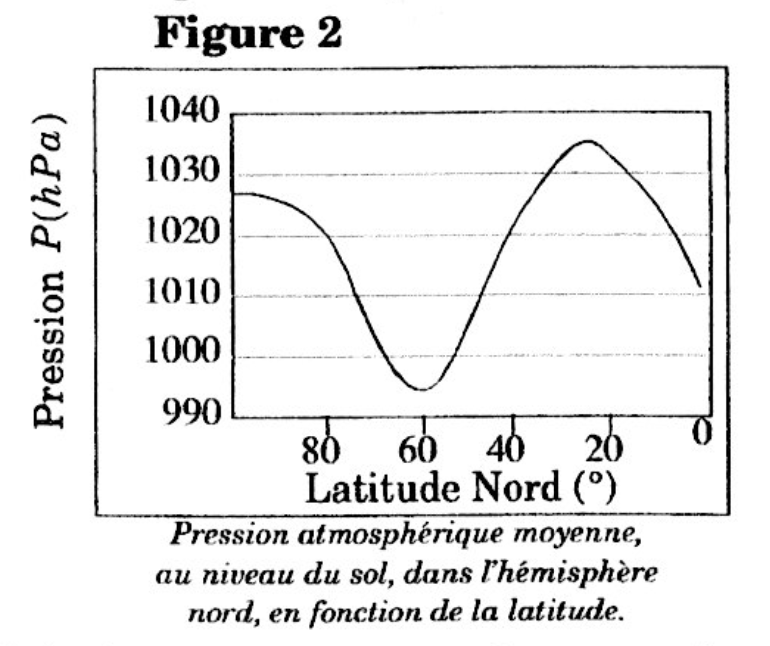
\includegraphics[scale=0.3]{meca_flu5bis.png}
\end{center}	
	
	\item[$\clubsuit$] Estimer la valeur typique de la vitesse des vents dominants en Europe.

\end{itemize}

\textit{Données} : $R_T=6370$km, $\Omega=2\pi/86164$rad.s$^{-1}$, $M=29$g.mol$^{-1}$.

\end{document}
